\chapter{Genifer 4.0}
\begin{flushright}
\english{blah}\\ --- blah
\end{flushright}
\minitoc

\section{Algebraic logic}

My motivation for studying algebraic logic is to develop better inference and learning algorithms for logic.  In the 1990s, the invention of SVMs by Vapnik revolutionized the field of statistical learning, and SVMs remain to be the best general spatial learner today.  What if we can invent something similar to logic as what SVM is to spatial domains?

\subsection{Survey of algebraic logic}

\citep*{Halmos1962}, \citep*{Andreka2001}, \citep*{Halmos1988}, \citep*{Craig1974}, \citep*{Plotkin1994}, \citep*{Lawvere2003}'s Appendix A.

\todo{Lawvere's idea that the existential and universal quantifiers are adjuncts to each other.  What use is it?}

\subsection{Speeding up inference and learning}

For all logics that I know of, deduction is performed by \textit{iterating} deductive steps.  Each step is the application of an inference rule.  If a formula with quantification is involved, some kind of pattern matching or unification is required apply the formula.  Such an iterative process is equivalent t o searching in a large proof space.

My idea is:  perhaps we can ``map'' logic to some \textit{continuous} space, and somehow approximate the proof process by spatial computational techniques?

One natural idea is:

\tab \begin{tabular}{rll}
first-order objects & $\longrightarrow$ & points in space\\
predicates          & $\longrightarrow$ & regions / shapes in space\\
logical entailment  & $\longrightarrow$ & finding intersections of regions\\
\end{tabular}

\begin{figure}[H]
\centering
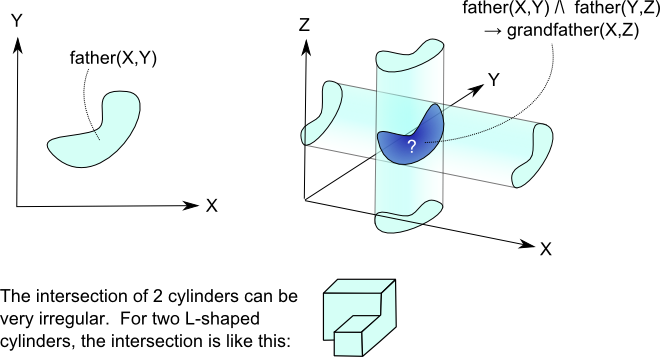
\includegraphics[scale=1.0]{cylindrical-logic.png}
%\caption{algebraic logic}
\end{figure}

We know that, for some concepts (predicates), the shape of the regions defining the predicate can be extremely irregular or even incomputable.

Our motivation is twofold:\\
1. How can we find intersections of regions efficiently?\\
2. Can we altogether avoid performing deduction via iterative steps?

One idea is to have multiple ``domain grids''.  We'd be sorting the source domains into various clusters.  That will speeed up the look-up of intersections.

However, this idea only gives us a geometric interpretation, but it doesn't tell us how to compute the shapes of regions efficiently.  The only way to compute the regions is to go back to the basic inference rules of the logic, ie, iteratively and syntactically.

Another idea is the ``dual'':

\tab \begin{tabular}{rll}
first-order objects & $\longrightarrow$ & shapes / regions in space\\
predicates          & $\longrightarrow$ & points in space\\
logical entailment  & $\longrightarrow$ & ?\\
\end{tabular}

\section{Genifer 4.0 理论}

Make the correspondence:
\begin{center}
\begin{tabular}{ccc}
logic formulas & $\Leftrightarrow$ & algebra over the ring of truth values \\
KB & $\Leftrightarrow$ & formal series \\
rule & $\Leftrightarrow$ & operator \\
pattern matching & $\Leftrightarrow$ & filter: KB $\rightarrow$ KB \\ 
deduction & $\Leftrightarrow$ & apply operators \\
learning & $\Leftrightarrow$ & find operator \\ 
\end{tabular}
\end{center}

\subsection{逻辑推导}

\subsection{学习}

% \setmainfont{SimSun}

学习的目的是寻找一组逻辑\  formulas 去解释这世界。  所谓解释即推导。

学习的方法是\  inductive learning,即由事实诱导出法则\  (induce rules from facts)。 Rules 就是逻辑範式。

Induction 需要的是一个\  general-to-specific order。  传统逻辑中这个序由两方面达成:
\begin{enumerate}
\item 某个\  concept 比另一个\  concept 更一般,例如: 动物/狗
\item conjunctions 的增加,例如: 戴眼镜\  $\wedge$ 长头发
\end{enumerate}

压缩的方法必须是\  ``semantic distance preserving'',意即: 在语义空间中相似的点被压缩到相邻的逻辑範式。

Gradient descent 的原理是我们必须知道\  $\frac{\partial\mathcal{E}}{\partial\mathbf{r}}$ 的值,其中 $\mathcal{E}$ 是误差,$\mathbf{r}$ 是法则空间中的座标。

误差\  $\mathcal{E}$ 由下式给出:
$$ \mathcal{E} = || R^\infty(\mathcal{F}) - \mathcal{F}^* || $$ 
$\mathcal{F}$ 是已知事实,$\mathcal{F}^*$ 是新的要学习的事实,$R$ 是所有法则,$r \in R$。

问题似乎是: 法则的诱导似乎不能单是基於语法。 概念阶层的诱导是基於: Liebniz 和\  $a R b$。

Liebniz extensionality:
\begin{eqnarray}
xZ \rightarrow yZ \Leftrightarrow x \supset y \\
Zx \rightarrow Zy \Leftrightarrow x \supset y
\end{eqnarray}

There are 2 ways to generalize a logic formula:
\begin{enumerate}
\item adding \textbf{conjunctions}
\item using concepts that admit \textbf{substitutions}
\end{enumerate}

The relation of subsumption is \textit{intrinsic} to the logic.  

\familydefault